
\section*{CHƯƠNG 1 - TỔNG QUAN ĐỀ TÀI}
\addcontentsline{toc}{section}{\numberline{}CHƯƠNG 1 - TỔNG QUAN ĐỀ TÀI}
\setcounter{section}{1}
\setcounter{subsection}{0}
\setcounter{figure}{0}
\setcounter{table}{0}

\subsection{Giới thiệu}
Trong kỷ nguyên số hiện nay, mạng xã hội và các nền tảng chia sẻ video như YouTube đã trở thành nguồn dữ liệu khổng lồ chứa đựng ý kiến, cảm xúc và phản hồi của người dùng về các sản phẩm, dịch vụ và nội dung giải trí. Đặc biệt trong ngành công nghiệp điện ảnh, các bình luận trên YouTube trailer phim cung cấp thông tin quý giá về phản ứng của khán giả trước khi phim được phát hành chính thức.

Phân tích cảm xúc (Sentiment Analysis) là một lĩnh vực quan trọng của xử lý ngôn ngữ tự nhiên (NLP - Natural Language Processing), cho phép máy tính hiểu và phân loại cảm xúc trong văn bản. Việc áp dụng phân tích cảm xúc vào dữ liệu bình luận YouTube giúp các nhà sản xuất phim, nhà phân phối và các nhà nghiên cứu thị trường hiểu rõ hơn về phản ứng của khán giả, từ đó đưa ra các quyết định chiến lược phù hợp.

\begin{figure}[H]
\centering
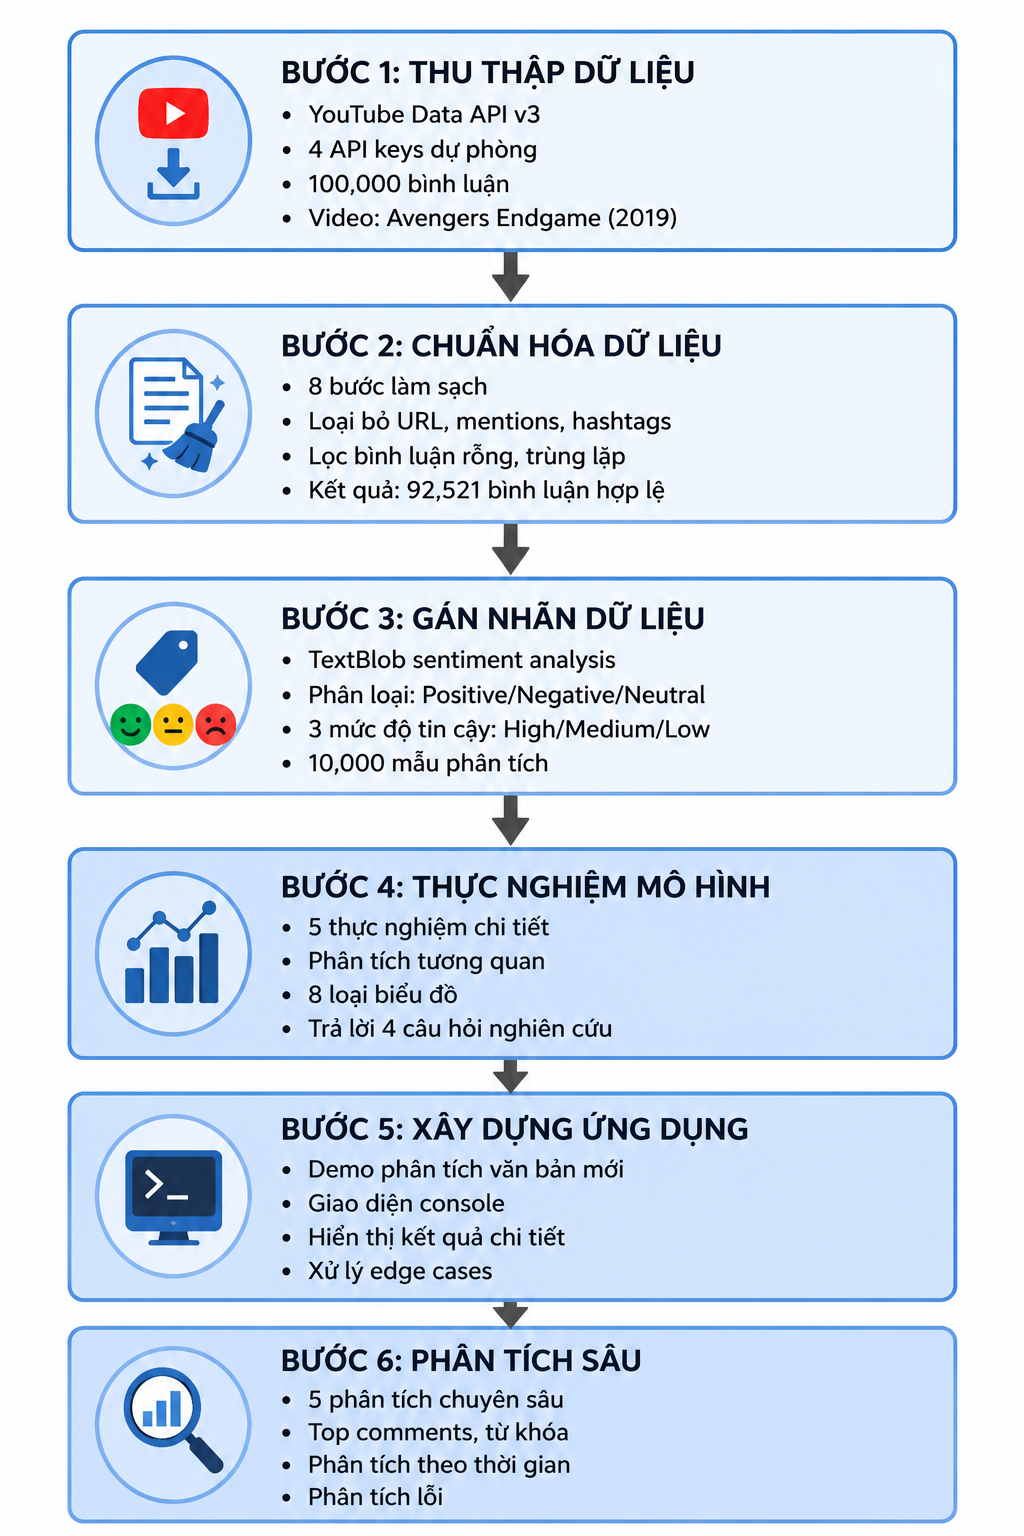
\includegraphics[width=0.85\textwidth]{image/sentiment_analysis_overview.png}
\caption{Quy trình phân tích cảm xúc bình luận YouTube}
\label{fig:sentiment_overview}
\end{figure}

Đề tài này tập trung vào việc xây dựng một hệ thống hoàn chỉnh để thu thập, chuẩn hóa và gán nhãn cảm xúc cho dữ liệu bình luận phim từ YouTube. Hệ thống sử dụng YouTube Data API v3 để thu thập dữ liệu quy mô lớn (hơn 100,000 bình luận), sau đó áp dụng các kỹ thuật tiền xử lý dữ liệu và thuật toán phân tích cảm xúc để phân loại bình luận thành ba nhãn: Tích cực (Positive), Tiêu cực (Negative) và Trung lập (Neutral).

\subsection{Lý do chọn đề tài}
Việc lựa chọn đề tài "Phân lớp Sentiment Analysis với YouTube API: Thu thập, chuẩn hóa và gán nhãn dữ liệu bình luận phim" xuất phát từ những lý do sau:

\textbf{Tính thực tiễn cao:} Phân tích cảm xúc là một trong những ứng dụng phổ biến nhất của Machine Learning và NLP trong thực tế. Các doanh nghiệp, đặc biệt trong ngành giải trí, marketing và thương mại điện tử, thường xuyên cần phân tích ý kiến khách hàng để đưa ra quyết định kinh doanh.

\textbf{Công nghệ tiên tiến:} Đề tài kết hợp nhiều công nghệ hiện đại bao gồm API Integration, Text Processing, Machine Learning và Data Visualization.

\textbf{Quy mô dữ liệu lớn:} Đề tài xử lý dữ liệu quy mô lớn (100,000+ bình luận) với hệ thống API dự phòng.

\textbf{Kỹ năng thực hành:} Đề tài yêu cầu triển khai hệ thống hoàn chỉnh từ đầu đến cuối (end-to-end).

\subsection{Mục tiêu nghiên cứu}
\textbf{Mục tiêu học thuật:}
\begin{itemize}
    \item Nghiên cứu và nắm vững các khái niệm về Sentiment Analysis và NLP
    \item Hiểu rõ quy trình thu thập dữ liệu từ API
    \item Phân tích các kỹ thuật tiền xử lý văn bản
\end{itemize}

\textbf{Mục tiêu kỹ thuật:}
\begin{itemize}
    \item Xây dựng hệ thống thu thập dữ liệu tự động với 4 API keys dự phòng
    \item Triển khai pipeline xử lý dữ liệu với 8 bước làm sạch
    \item Phát triển thuật toán phân loại cảm xúc với 3 mức độ tin cậy
\end{itemize}

\subsection{Phạm vi nghiên cứu}
Đề tài tập trung vào:
\begin{itemize}
    \item Thu thập dữ liệu từ YouTube API v3
    \item Xử lý và chuẩn hóa dữ liệu văn bản tiếng Anh
    \item Phân loại cảm xúc thành 3 nhãn: Positive, Negative, Neutral
    \item Phân tích và trực quan hóa kết quả
\end{itemize}

\subsection{Cấu trúc dự án và mã nguồn}

\subsubsection{GitHub Repository}
Toàn bộ mã nguồn và dữ liệu của dự án được công khai trên GitHub:

\textbf{Repository:} \url{https://github.com/0785420667nguyen-art/Final_Datamining_52300230_52300130}

\textbf{Cấu trúc thư mục:}
\begin{verbatim}
Final_Datamining_52300230_52300130/
├── data/                      # Dữ liệu và kết quả
│   ├── youtube_raw_data.csv       # Dữ liệu thô (88,969 rows)
│   ├── youtube_clean_data.csv     # Dữ liệu sạch
│   ├── youtube_labeled_data.csv   # Dữ liệu đã gán nhãn
│   ├── distribution.png           # Biểu đồ phân bố
│   ├── analysis.png               # Biểu đồ phân tích
│   └── README.md                  # Hướng dẫn về dữ liệu
├── source/                    # Mã nguồn
│   ├── sentiment_analysis.py      # Code chính (6 bước)
│   ├── app.py                     # Web App (Flask)
│   ├── get_examples.py            # Script lấy ví dụ
│   ├── templates/
│   │   └── index.html            # Giao diện web
│   ├── run.bat                    # Chạy dự án chính
│   ├── run_app.bat                # Chạy web app
│   └── README.md                  # Hướng dẫn về code
├── 52300230/                  # Báo cáo LaTeX
│   ├── main.tex
│   ├── chuongs/
│   └── image/
├── requirements.txt           # Thư viện Python
├── .gitignore                 # Git ignore
└── README.md                  # Hướng dẫn tổng quan
\end{verbatim}

\subsubsection{Vị trí dữ liệu và mã nguồn}
\textbf{Folder data/:} Chứa tất cả dữ liệu thu thập và kết quả phân tích
\begin{itemize}
    \item 3 file CSV: raw, clean, labeled (tổng 88,969 bình luận)
    \item 2 file PNG: biểu đồ phân bố và phân tích
    \item README.md: Mô tả chi tiết về dữ liệu
\end{itemize}

\textbf{Folder source/:} Chứa toàn bộ mã nguồn Python
\begin{itemize}
    \item sentiment\_analysis.py: Code chính (6 bước pipeline)
    \item app.py: Web application với Flask
    \item get\_examples.py: Script lấy ví dụ từ dữ liệu
    \item templates/: Giao diện HTML cho web app
    \item run.bat, run\_app.bat: Scripts chạy nhanh
    \item README.md: Hướng dẫn sử dụng code
\end{itemize}

\subsubsection{Hướng dẫn sử dụng}
\textbf{Clone repository:}
\begin{verbatim}
git clone https://github.com/0785420667nguyen-art/
    Final_Datamining_52300230_52300130.git
cd Final_Datamining_52300230_52300130
\end{verbatim}

\textbf{Cài đặt thư viện:}
\begin{verbatim}
pip install -r requirements.txt
\end{verbatim}

\textbf{Chạy dự án chính:}
\begin{verbatim}
cd source
python sentiment_analysis.py
\end{verbatim}

\textbf{Chạy web app:}
\begin{verbatim}
cd source
python app.py
# Truy cập: http://localhost:5000
\end{verbatim}

\subsection{Cấu trúc báo cáo}
\textbf{Chương 1:} Tổng quan đề tài - Giới thiệu, mục tiêu, phạm vi, cấu trúc dự án

\textbf{Chương 2:} Cơ sở lý thuyết - Sentiment Analysis, NLP, YouTube API, TextBlob

\textbf{Chương 3:} Thiết kế hệ thống - Kiến trúc, module, cấu trúc dữ liệu, ứng dụng demo

\textbf{Chương 4:} Triển khai và đánh giá - Môi trường, kết quả, thực nghiệm, phân tích sâu

\textbf{Chương 5:} Kết luận và hướng phát triển - Tổng kết, đánh giá, bài học, hướng phát triển
